\chapter{Long-read Sequencing}\label{ch: long_read_sequencing}

This chapter provides a detailed background into the two main platforms of long-read cDNA sequencing that were used in this thesis: Pacific Bioscience's Isoform Sequencing (Iso-Seq) and Oxford Nanopore Technology's cDNA sequencing.  

\section{Pacific Biosciences: Isoform Sequencing}
\label{sec:pb_isoform_sequencing}

\subsection{Introduction}
For successful DNA polymerisation, the DNA polymerase requires high concentration of nucleotides to allow high accuracy and processivity. However for sequencing, this limits sensitivity to detect each labelled base incorporation and respective fluorophore emission, due to high background noise level. Historically, second-generation sequencing technologies such as Illumina RNA-Sequencing have circumvented this issue by the step-wise addition, scan and wash of each set of labelled nucleotides, but at a compromise of read length (discussed in \cref{rnaseq_intro}). 

Unlike standard approaches of RNA-Sequencing, Pacific Bioscience’s Single Molecule Real Time sequencing (SMRT\nomenclature{SMRT}{Single Molecule Real Time sequencing}) is able to generate long reads is due to its ability to mimic natural, uninterrupted, processive DNA synthesis, through three important innovations \cite{Eid2009}: 
\begin{enumerate}
	\item Creation of a circular template, SMRTbell, enclosed with hairpin adapters at end of the inserted target double-stranded DNA, allowing uninterrupted DNA polymerisation \cite{Travers2010} (\cref{fig:Mechanism}\textbf{a}).
	\item Sequencing of each SMRTbell with a bound polymerase at the bottom of a nanometre-wide well (zero-mode-waveguide - ZMW\nomenclature{ZMW}{Zero-Mode-Waveguide}), and all wells contained within a single SMRT chip\cite{Levene2003}. Due to the very nanoscale size of the ZMW and reduced detection volume, a single nucleotide incorporation can be sensitively detected against the high background of labelled nucleotides, achieving a high-signal-to-noise ratio (\cref{fig:Mechanism}\textbf{b}). PacBio currently offers two sequencers, which primarily differs in the number of ZMWs: Sequel I with 1M ZMWs and Sequel II with 8M ZMWs.   
	\item Addition of phospholinked nucleotides, each labelled with a different colour fluorophore corresponding to the four different bases (A, C, G and T), which allows for natural, accurate and processive DNA synthesis\cite{Mccarthy2010} (\cref{fig:Mechanism}\textbf{c}).
\end{enumerate}
In summary, PacBio SMRT sequencing detect fluorescence events that correspond to addition of one specific nucleotide by a polymerase attached to the bottom of a tiny well. 


\begin{figure}[h!]
	\centering
	\includegraphics[page=14,trim={0 5cm 0 0 },clip, scale = 0.7]{Figures/ProjectDevelopment_Figures.pdf}
	\captionsetup{width=0.95\textwidth}
	\caption[Pacific Bioscience's Single Molecule Real-time Sequencing]%
	{\textbf{Pacific Bioscience's Single Molecule Real-time Sequencing (SMRT)}: PacBio's SMRT technology is able to generate long reads >10kb by \textbf{a)} enclosing the cDNA fragment of interest within a circular template (SMRTbell") to allow interrupted DNA polymerisation, \textbf{b)} sequencing of each SMRTbell with a bound polymerase at the bottom of ZMWs, enabling sensitive detection of polymerisation at nucleotide level, and \textbf{c)} addition of phospholinked nucleotides with differently labelled fluorophore. ZWW - Zero-Mode-Waveguide}
	\label{fig:Mechanism}
\end{figure}


\subsubsection{Mechanism}
Due to the circular nature of the SMRTbell template, the polymerase is able to continually read through the insert in an interrupted fashion multiple times (or "passes"), resulting in a continuous read (known as polymerase read) (\cref{fig:Mechanism}\textbf{a}). In removing the hairpin-adapters that delineate the repeated insert sequence, this polymerase read is then resolved to multiple reads (known as subreads), which are then further merged to yield one high-quality and highly-accurate consensus read (known as Circular Consensus Sequence - CCS\nomenclature{CCS}{Circular Consensus Sequence}) (\cref{fig:Mechanism}\textbf{a}). Dependent on the polymerase lifetime and insert length and, the generation of CCS can increase the accuracy from 85\% (raw subreads) to 99\%, proportional to the number of passes \cite{Travers2010}. 

Consequently, unlike short-reads generated by RNA-Seq, PacBio Iso-Seq reads are not of a set length, but cover a range of lengths that is dependent on the library size and the polymerase activity\cite{Ardui2018,Rhoads2015}. With previous chemistries, there was a bias towards sequencing molecules of a certain length due to preferential loading of SMRTbell templates - Diffusion Loading favoured shorter molecules\cite{Loomis2013} whereas Magbead Loading allowed proportional loading to the concentration rather than by length, but prevented sequencing of molecules <1kb (discussed in \cref{section:ch2_polbinding_loading}). Previous attempts to mitigate this loading challenge have been to fractionate the library by length (size selection) and enrich for longer cDNA molecules before sequencing\cite{Au2013}, but this approach is more expensive and laborious. Thankfully, recent improvements in both technology and chemistry with usage of molecular crowding agents have alleviated the sequencing read bias and resulting the Magbead loading method obsolete \cite{Oikonomopoulos2020}.   


\subsubsection{Performance and Run Quality Metric}
Suboptimal sequencing performance could be due to various reasons from potential issues with the instrument and sequencing reagents, to poor library preparation and incorrect loading. Evaluation of the performance of the DNA Internal Control (described in \cref{section:ch2_sequencing}) and productivity metrics would provide useful insights into the performance of a sequencing run. 

\boldheader{DNA Internal Control} 
Sequencing metrics for the DNA Internal Control (described in \cref{section:ch2_sequencing}) include: i) the number of control reads, ii) the mean polymerase read length of the control and iii) the proportion of identity match between the control raw reads and the control reference sequence (concordance). The expected values from a correctly prepared control in a sequencing run, with a 4hr pre-extension time and a 20hr capture time is documented in \cref{tab:control_Isoseqmetrics}. Low control read length and/or low control read counts suggest issues with the PacBio instrument and consumables, whereas expected values indicate sample-specific issues. The concordance value is a useful metric for optimum loading whereby over-loaded SMRT cells would typically have a lower value (<0.84).

\begin{table}[!h]
	%\captionsetup{justification=raggedright,width=1.45\textwidth}
	\caption[Iso-Seq DNA Internal Control Sequencing Metrics]%
	{\textbf{Iso-Seq DNA Internal Control Sequencing Metrics.} The expected median values for the number of control reads (median count), the control polymerase read length (median length), and the identity match between control raw reads and reference sequence (median concordance). The expected values shown are assuming a sequencing run performed with SMRT cells 1M v3 with Sequel DNA Internal Control Complex, Sequel Sequencing Kit 3.0 on the Sequel I with a 4hr pre-extension time of 4hrs and a 20hr capture time.}
	\label{tab:control_Isoseqmetrics}
	
	\centering
	\begin{tabular}{@{}cccc@{}}
		\toprule
		Metrics         & Median Count (QR)     & Median Length (kb) (QR) & Median Concordance (QR) \\ \midrule
		Expected Values & 6900 (4,000 - 10,200) & 46.9 (41.5 – 52.5) & 0.862 (0.857 – 0.867)   \\ \bottomrule
	\end{tabular}
\end{table}


\boldheader{Productivity Metrics} 
Productivity or loading metrics is a measure of the number of ZMWs that have generated a positive signal and subsequently, useful sequencing data. Each ZMW is classified as either: 
\begin{itemize}
	\item P0 (Productivity 0): no active sequencing polymerase complex with no signal 
	\item P1 (Productivity 1): productive ZMWs with a high quality (HQ) region within read 
	\item P2 (Productivity 2): detectable signal but no HQ region detected, possibly due to overloading of multiple inserts with multiple polymerases
\end{itemize}
High quality region is defined as a high quality sequence of >50bases. These metrics are also dependent on chemistry, pre-extension, and movie runtime.  

An optimal sequencing run is indicated by a 20-30\% P0 (proportion of empty ZMWs). A lower P0 (<20\%) from over-loading of polymerase-bound complexes on SMRT cells would result in poorer sequencing yield (noisy base-calling) and shorter P1 polymerase reads, whereas, a higher P0 (>40\%) from under-loading would result in fewer P1 reads and subsequently lower sequencing yield. Of note, a combination of high P0, low P1 and high P2 loading profile indicates presence of contaminants (possibly due to poor AMPure bead purification) that is interfering with productive polymerase activity. A good balance between P0, P1 and P2 is therefore critical and can be achieved by determining an optimum loading concentration through performing titrations of multiple loading concentrations.

\subsection{Lab Workflow}
\label{chap:isoseq_labpipeline}
This section specifically describes the lab workflow for the library preparation for PacBio Iso-Seq. All details relating to sample preparation, cDNA synthesis and amplification can be found in \cref{ch: general methodology}.

The Iso-Seq lab protocol, as outlined in \cref{fig:isoseq_wholelab_protocol}, involved three main steps by i) converting total RNA transcripts to full-length cDNA using the Clontech SMARTer PCR cDNA synthesis kit, ii) amplification and purification of double-stranded cDNA, and iii) performing library preparation for long-read sequencing which involved constructing the SMRT bell library. Size selection was not performed with full-length transcript detection of up to 4 kB. For targeted transcriptome profiling with enrichment of target genes, all the steps in the workflow were identical with an additional step of target capture post ds-DNA amplification and pre-SMRT bell library, and usage of barcodes to allow multiplexing (\cref{fig:isoseq_targetedlab_protocol}). 

\begingroup
\parindent=0em
\etocsettocstyle{\rule{\linewidth}{\tocrulewidth}\vskip0.5\baselineskip}{\rule{\linewidth}{\tocrulewidth}}
\etocsetnexttocdepth{5}
\localtableofcontents 
\endgroup

\begin{figure}[htp]
	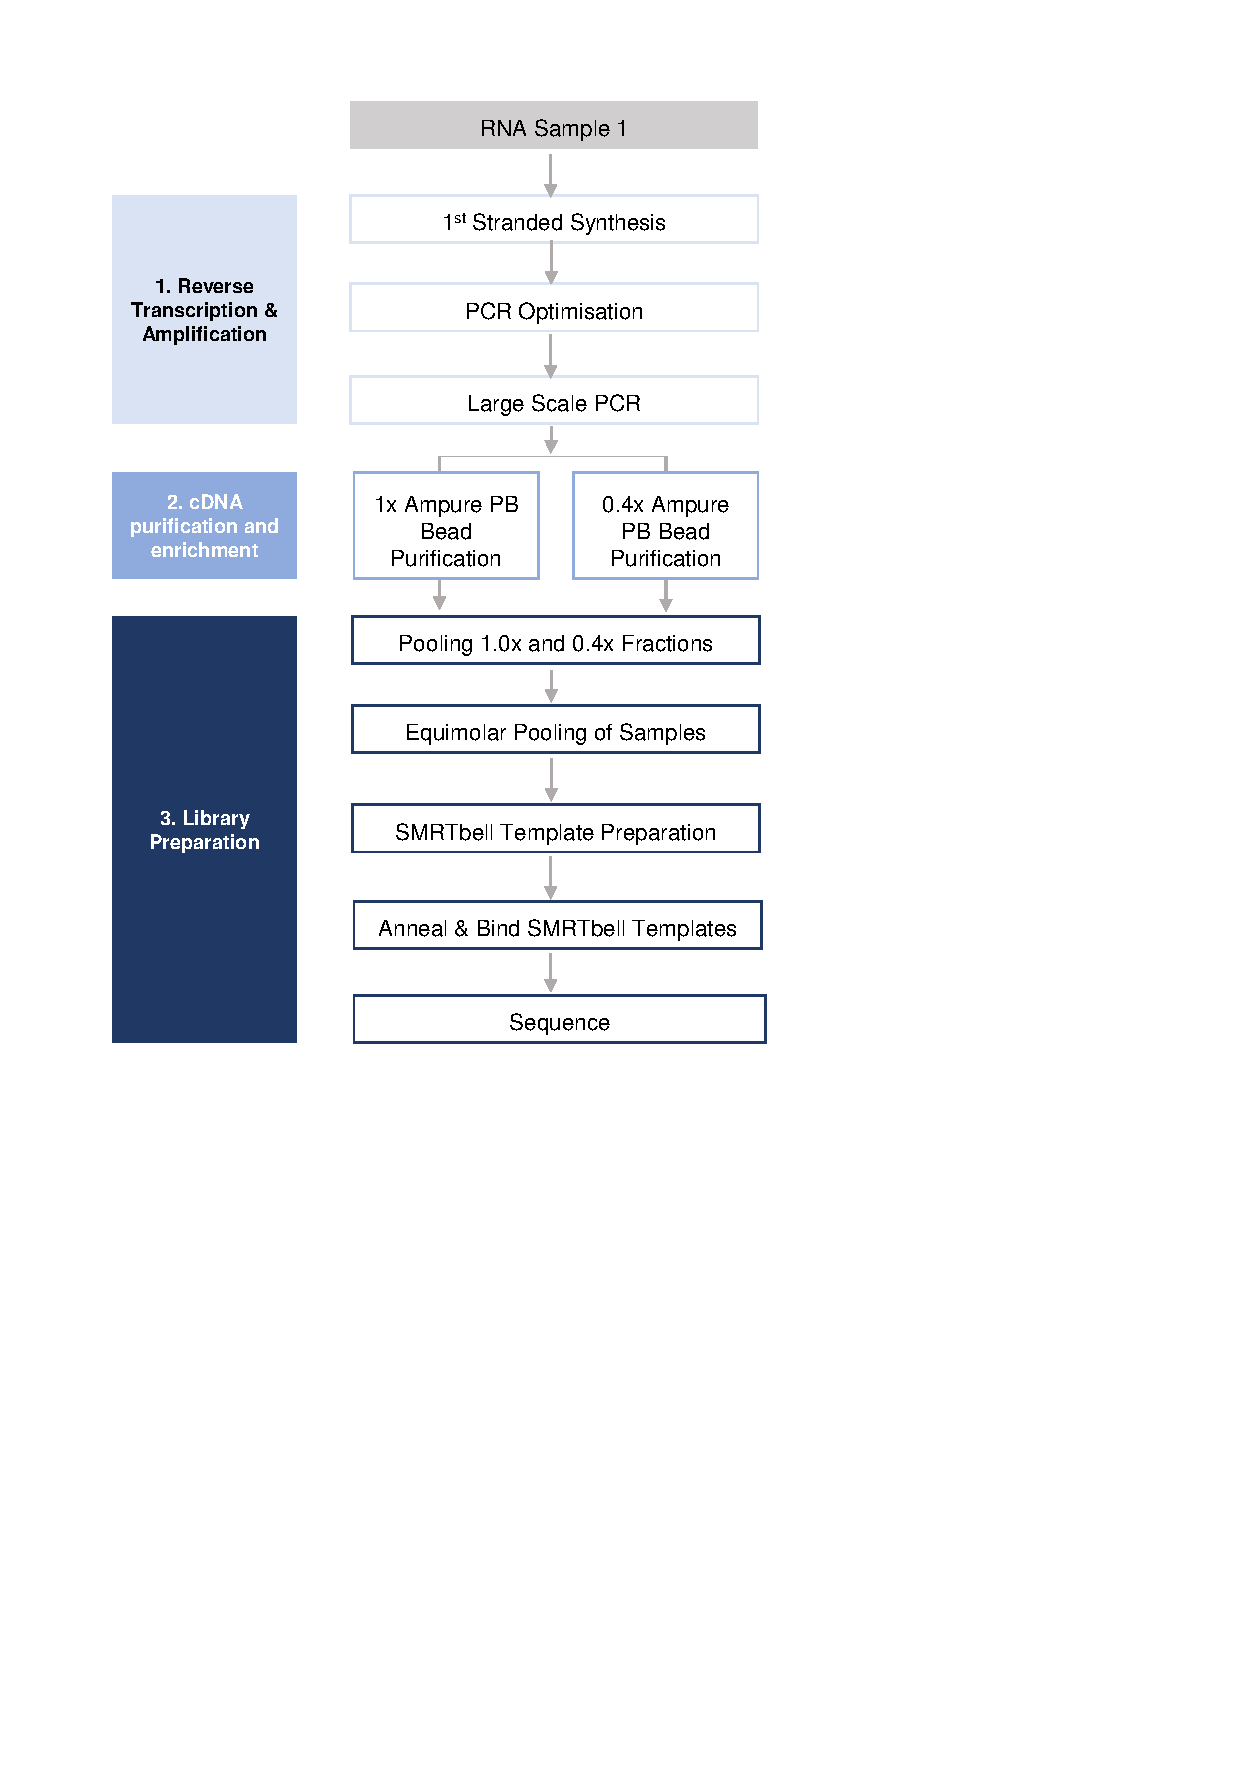
\includegraphics[page=1,trim={0 12cm 5cm 1cm},clip,scale = 1]{Figures/ProjectDevelopment_Figures.pdf}
	\captionsetup{width=0.95\textwidth}
	\caption[Iso-Seq Lab workflow used for whole transcriptome sequencing]%
	{\textbf{An overview of the lab Iso-Seq workflow used for whole transcriptome profiling}. The lab workflow, as adapted from official Iso-Seq protocol, involves three main steps: 1) reverse transcription and amplification of cDNA ( \cref{section:ch2_cDNA_synthesis_explanation}), 2) cDNA purification with AMPure beads ( \cref{section:ch2_AMPure_explanation}) and 3) library preparation involving ligation of SMRT bell templates, and primer and polymerase binding (\cref{section:ch2_smrtbelltemplate_explanation})}
	\label{fig:isoseq_wholelab_protocol}
\end{figure}

\begin{figure}[]
	\begin{center}
		\includegraphics[page=2,trim={1cm 12cm 1cm 1cm},clip,scale = 0.8]{Figures/ProjectDevelopment_Figures.pdf}
	\end{center}
	\captionsetup{width=0.95\textwidth}
	\caption[Iso-Seq Lab workflow used for targeted transcriptome sequencing]%
	{\textbf{An overview of the lab Iso-Seq pipeline used for targeted transcriptome profiling}. The lab workflow for targeted transcriptome profiling involves all the steps in the standard Iso-Seq lab workflow (Figure \ref{fig:isoseq_wholelab_protocol}), with the addition of the target capture step (Boxed orange, Section \ref{section:ch2_targetcapture_explanation}) and the use of barcoded primers in reverse transcription (Boxed green and denoted here as Barcode 1 and Barcode n) to allow sample multiplexing (denoted here as Sample n, PacBio recommends 6-8 multiplexed samples per run). The list of barcodes can be found in \cref{tab:barcode_primers}}
	\label{fig:isoseq_targetedlab_protocol}
\end{figure}


\subsubsection{PCR optimisation and DNA Amplification}
\label{ch: pcr_optimisation}
After cDNA synthesis (described in \cref{section:ch2_cDNA_synthesis_explanation}), cDNA products were amplified using PCR (described in \cref{section:ch2_PCR_explanation}) to ensure sufficient material for sequencing. To minimise PCR bias (under or over-amplification), which can result in under or over representation of the different cDNA library size, the optimal number of PCR cycles for amplification with PrimeSTAR GXL DNA Polymerase (Clontech) was determined (\cref{fig:pcr_optimisation_gel_eg}). This was achieved by collecting 5uL PCR aliquots every two cycles (cycle 10, 12, 14, 16, 18, 20) followed by visualisation of cDNA products on a 1.5\% Agarose gel electrophoresis with ethidium bromide. Large scale PCR amplification was then subsequently performed using the optimal number of cycles.

%Single-stranded DNA generated from SMARTer PCR synthesis kit in the official Iso-Seq protocol was amplified by PCR using PrimeSTAR GXL DNA Polymerase (ClonTech). Also performed for targeted sequencing. 

\begin{figure}[htp]
	\begin{center}
		\includegraphics[page=13,trim={1cm 24cm 10cm 1cm},clip,scale = 0.9]{Figures/ProjectDevelopment_Figures.pdf}
	\end{center}
	\captionsetup{width=0.95\textwidth}
	\caption[Example of Agarose gel to determine optimum number of PCR cycles for amplification]%
	{\textbf{PCR optimisation is required to determine optimum number of cycles}. Shown is an agarose gel of Human Brain Total RNA after 1st strand cDNA synthesis and PCR amplification through cycles 8 to 18, with PCR aliquots collected during respective cycles. In this example, 10 cycles were determined to be the optimum number for large-scale amplification. While smear distribution from 8 and 10 cycles look similar, 10 cycles show more products thereby generating sufficient material for downstream pooling. Cycles above 12 show signs of over-amplification which will result in biased sequencing representation. Figure and legend are adapted from Iso-Seq protocol}
	\label{fig:pcr_optimisation_gel_eg}
\end{figure}


\subsubsection{AMPure Bead Purification} 
Post large scale amplification, the resulting PCR product was divided into two fractions and purified with 0.4X and 1X AMPure PB beads (PacBio), such double-stranded DNA was bound to the beads and isolated in either 1:1 or 1:0.4 ratio. DNA purification with 0.4X AMPure beads was important to ensure enrichment of longer fragments (as described in \cref{section:ch2_AMPure_explanation}) to provide a more representative sequencing library; Iso-Seq is length-biased as shorter fragments diffuse faster into ZMW and are therefore more likely to be sequenced. Quantification and size distribution of each fraction was then determined using Qubit DNA High sensitivity assay (Invitrogen) and Bioanalyzer assays on the 2100 Bioanalyzer (Agilent). Two fractions per sample were then recombined at equimolar quantities and library preparation performed using SMRTbell Template Prep Kit v1.0 (PacBio). 

The molarity was calculated by the following equation: 
\begin{equation}
	\label{eqn:isoseq_library_molarity}
	\frac{concentration(\frac{ng}{ul})\times 10^6}{660(\frac{g}{mol}) \times average\:library\:size\:in\:bp\mbox{*}} = concentration\;in\; nM
\end{equation}
* the average library size was determined by the start and end point of the smear

\subsubsection{Target Capture using IDT Probes} 
\label{section:ch2_targetcapture_explanation} 
For targeted sequencing, we used the official PacBio protocol “cDNA Capture Using IDT
xGen® Lockdown Probes” (an adaptation of the official IDT protocol “xGen hybridisation capture of DNA libraries” ), which slotted as an additional step to the standard protocol between cDNA amplification and ligation (\cref{fig:isoseq_targetedlab_protocol}). Enrichment of target genes involved hybridisation of dsDNA using pre-designed, complementary 5’ biotinylated DNA 120nt-long oligonucleotides (hereby referred as probes). The hybridised library fragments were then washed, isolated with magnetic streptavidin beads, amplified using Takara Hot-Start polymerase and then further purified with AMPure beads. After assessing the quality and quantity of the target cDNA using the Bioanalyzer and qubit, SMRT Bell template preparation, primer and polymerase annealing were proceeded according to the standard official Iso-Seq protocol. Given the samples were multiplexed for targeted sequencing, the samples were first pooled in equal molarity before probe hybridisation.  

%*Modifications to the protocol: waiting times at room temperature during hybridisation, lid heat temperatures, method of washing beads at room temperature; all modifications are incorporated from official IDT protocol, post amplification clean-up for consistency  

\myparagraph{Selection of probes}
Probes were designed to a panel of 20 AD-associated genes: \textit{Bin1, Trem2, Cd33, Vgf, Fyn, Mapt, Trpa1, Picalm, Sorl1, Abca7, Snca, Apoe, Abca1, App, Ank1, Clu, Fus, Ptk2b, Rhbdf2, Tardbp}. Two separate pools of the equal molar probes were created using the mouse (GRCm28/mm10) and human genome (GRCh37/hg19). While IDT provided a pre-designed set of probes to the target genes, many of them were found to overlap with the intronic regions of the target gene with contiguous coverage. 

Given that previous studies with targeted sequencing have found that the target gene can be successfully enriched with a few unique probes to the exonic regions, I manually assessed the list of probes for each target gene using the following criteria:
\begin{itemize}
	\item Ensured each exon in every gene is covered at least once (exons > 500bp has >1 probe) 
	\item Removed any probes to intronic regions
	\item Within each exon, removed any contiguous probes (as seen in the 1x tiling density) and ensured probes spaced 300-500bp (equivalent to 0.2x – 0.3x tiling density) 
	\item From the contiguous “cluster”, selected probes with the highest GC content (40-65\% GC content)/minimal number of blast hits 
\end{itemize}
The coverage of each target gene can be found in Appendix. 

\begin{figure}[!h]
	\begin{center}
		\includegraphics[page=12,trim={0cm 6cm 0cm 1cm},clip,scale = 0.70]{Figures/ProjectDevelopment_Figures.pdf}
	\end{center}
	\captionsetup{width=0.95\textwidth}
	\caption[Lab workflow for hybridisation capture of cDNA for targeted transcriptome profiling]%
	{\textbf{Lab workflow for hybridisation capture of cDNA for targeted transcriptome profiling.} An overview of the lab workflow of enrichment of target genes involving hybridisation of cDNA with probes and blockers (polyT oligonucleotide, cDNA synthesis primers), followed by capture with streptavidin beads. The addition of blockers prevent non-specific binding and subsequently increases enrichment sequencing depth}
	\label{fig:isoseq_targetcapture}
\end{figure}

\begin{landscape}
	\begin{figure}[ht]
		\begin{center}
			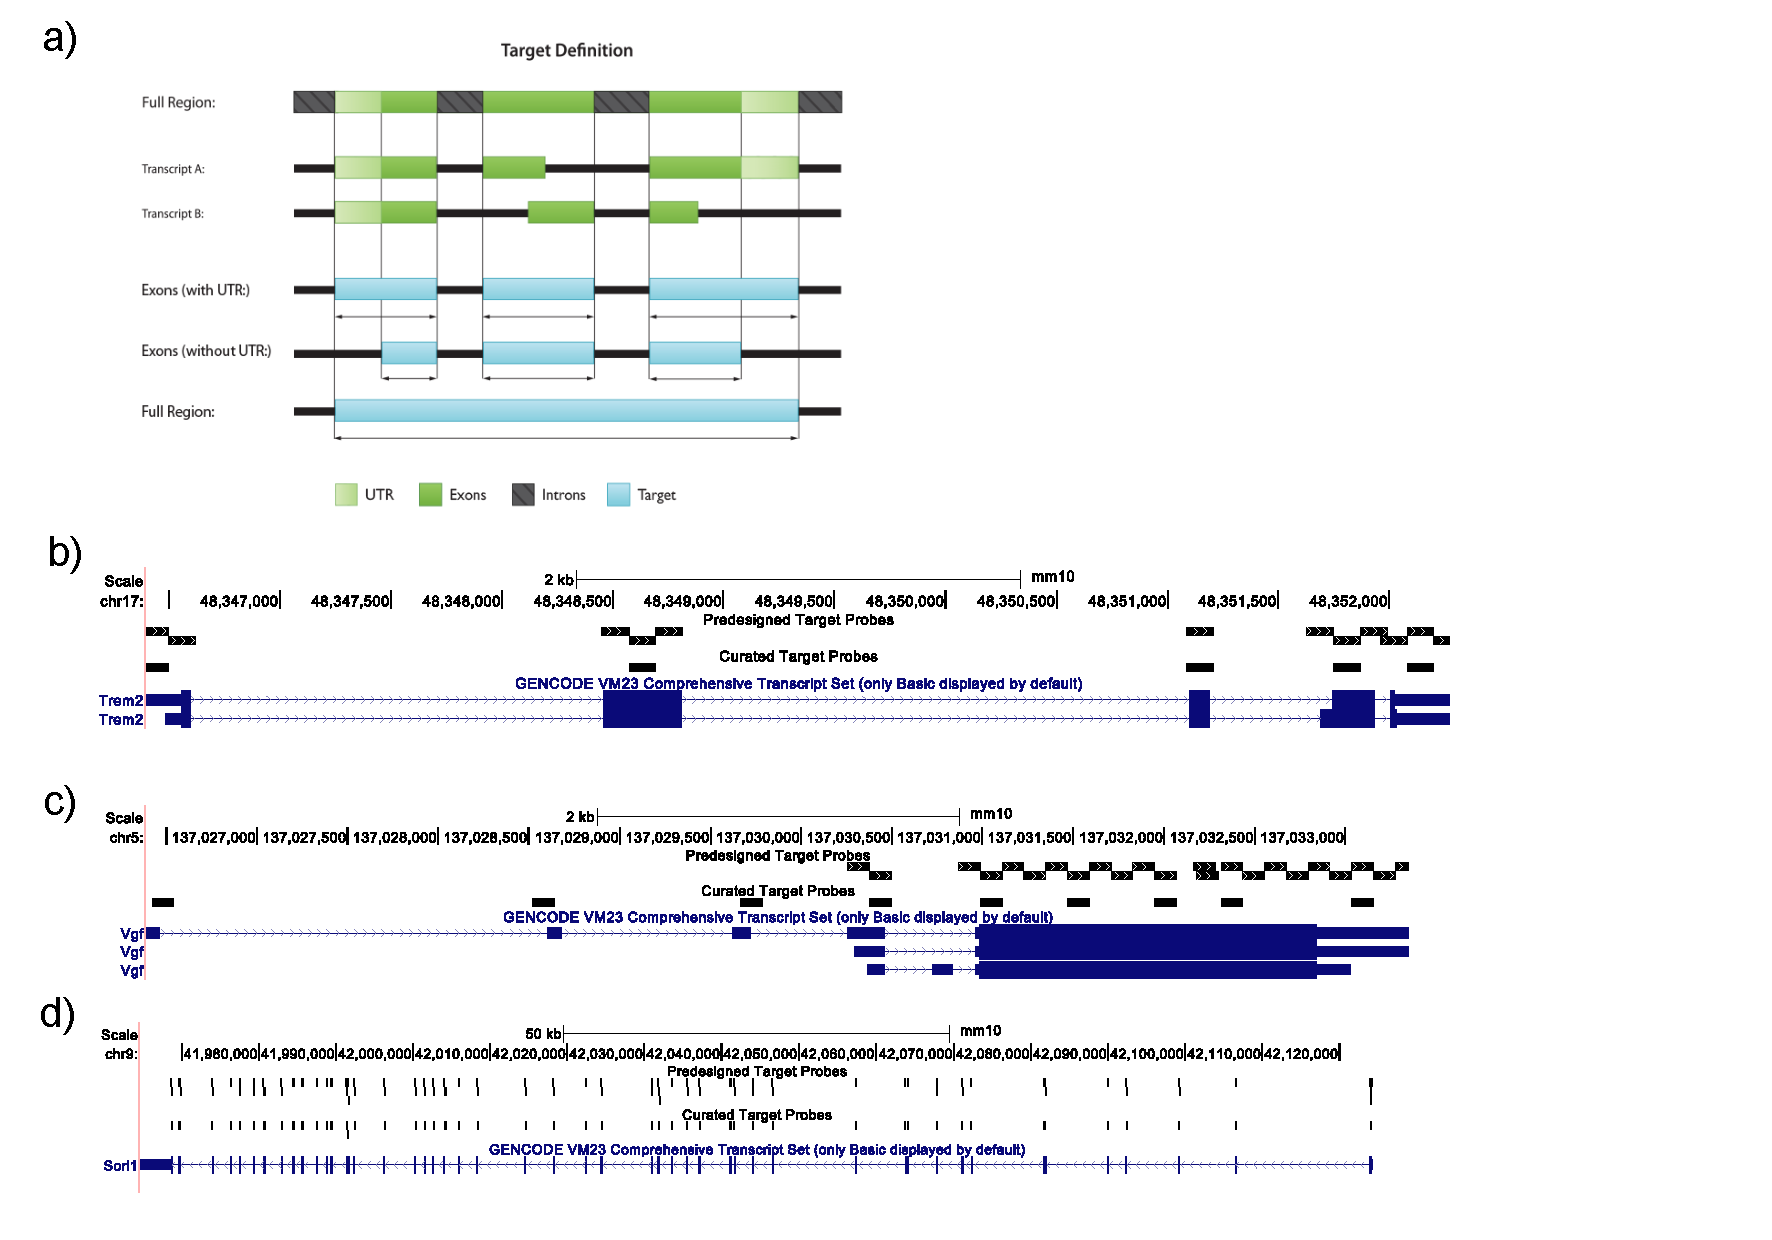
\includegraphics[page=1,trim={0cm 2cm 0cm 0cm},clip,scale = 0.70]{Figures/TargetProbes_Visualisation.pdf}
		\end{center}
		\captionsetup{width=1.5\textwidth}
		\caption[Manual curation of probes designed to 20 AD-associated target genes]%
		{\textbf{Manual curation of probes designed to 20 AD-associated target genes.} \textbf{a)} Pre-designed set of probes were provided to "Exons (without UTR)" of target genes. However, exons were unnecessarily covered by contiguous probes which not increases costs but also off-target binding (referred in figure as Pre-designed Target Probes). Manual curation was therefore needed for each target gene (referred in figure as Curated Target Probes))to ensure that only exons are covered with one probe for every 500bp. Shown in \textbf{b,c,d)} are UCSC genome browser tracks of pre-designed and curated probes to \textit{Trem2}, \textit{Vgf} and \textit{Sorl1} in mouse genome. }
		\label{fig:target_probes_eg}
	\end{figure}
\end{landscape}

\subsubsection{SMRT Bell Template Preparation}
\label{section:ch2_smrtbelltemplate_explanation} 
After pooling the two fractions at equimolar quantities with the SMRTbell Template Prep Kit v1.0 (PacBio), SMRT bell template preparation was performed (\cref{fig:isoseq_labworkflow}, Step 1, 2). This involved repairing DNA damage and polishing ends of fragments for ligation of blunt hairpin adapters, essential to generate high quality library of closed, continuous and circular SMRTbell templates. Any abasic sites were filled-in, thymine dimers resolved, and deaminated cytosine are alkylated. 3’ overhangs were removed, whereas 5’ overhangs were filled-in by T4 DNA Polymerase and phosphorylated by T4 PNK. Following 1x AMPure purification of repaired dsDNA, hairpin adapters were then ligated to the blunt ends for up to 24hours (\cref{fig:isoseq_labworkflow}, Step 3). Any fragments failed to ligate were removed with exonuclease III and VII (\cref{fig:isoseq_labworkflow}, Step 4). The repaired, ligated SMRT bell library was then purified twice with 1x AMPure beads, and assessed with Qubit DNA High sensitivity assay (Invitrogen) and Bioanalyzer 2100 before proceeding to primer annealing and polymerase binding (\cref{fig:isoseq_labworkflow}, Step 5,6). 

\subsubsection{Primer Annealing and Polymerase Binding} 
\label{section:ch2_polbinding_loading}
Post ligation of hairpin adapters, sequencing primer and polymerase were bound to both ends of the SMRTbell templates. The primer and polymerase to template ratio was critical to minimise under- or –over loading, and is dependent on the loading method (Diffusion or Magbead), and concentration and mean library size. The SMRTbell molarity was determined using the previous \textbf{Equation \ref{eqn:isoseq_library_molarity}}.

Prior to the release of v3.0 chemistry in 2018, Magbead Loading was only recommended for Iso-Seq SMRTbell libraries, whereas Diffusion Loading was recommended for all other applications with insert sizes from 250bp – 100kb. As suggested by the name, Diffusion loading involves immobilization of polymerase-bound SMRTbells to ZMW by diffusion, whereas Magbead loading involves immobilization by attachment to paramagnetic beads. Magbead loading therefore requires an additional step of hybridising SMRTbell templates to Magbeads and washing of SMRTbell-bound Magbeads before loading on the instrument, whereby a built-in Magbead station facilitates movement of Magbeads across ZMW. Typically, Diffusion loading preferentially loads shorter transcripts, whereas Magbead loading preferentially loads longer >1b as it rolls across nanowells. However, with the newer release of kits and chemistry, diffusion loading was recommended for all applications including Iso-Seq. Subsequently, all of the samples bar the first two were sequenced by Diffusion Loading. 


\subsubsection{Sequencing} 
\label{section:ch2_sequencing}
Sequencing was performed on the PacBio Sequel 1M SMRT cell. Samples were processed using either the v3 chemistry (diffusion loading at 5pM, pre-extension 4 hours, Capture time 20 hours) or v2.1 chemistry (Magbead loading at 50pM with a 2 hour pre-extension and 10 hour capture).

Of note, DNA Internal Control Complex (PacBio) was also added to each library before sequencing. Composed of a 1966bp-insert that has already been ligated with SMRTbell adapters and bound by polymerase, this control sequence provides a quality-control measure of loading and sequencing performance. The amount of internal control was similarly determined by the library size and concentration, with PacBio recommending an average number of 500-1000 sequenced reads per SMRT cell.     

\begin{figure}[!htp]
	\begin{center}
		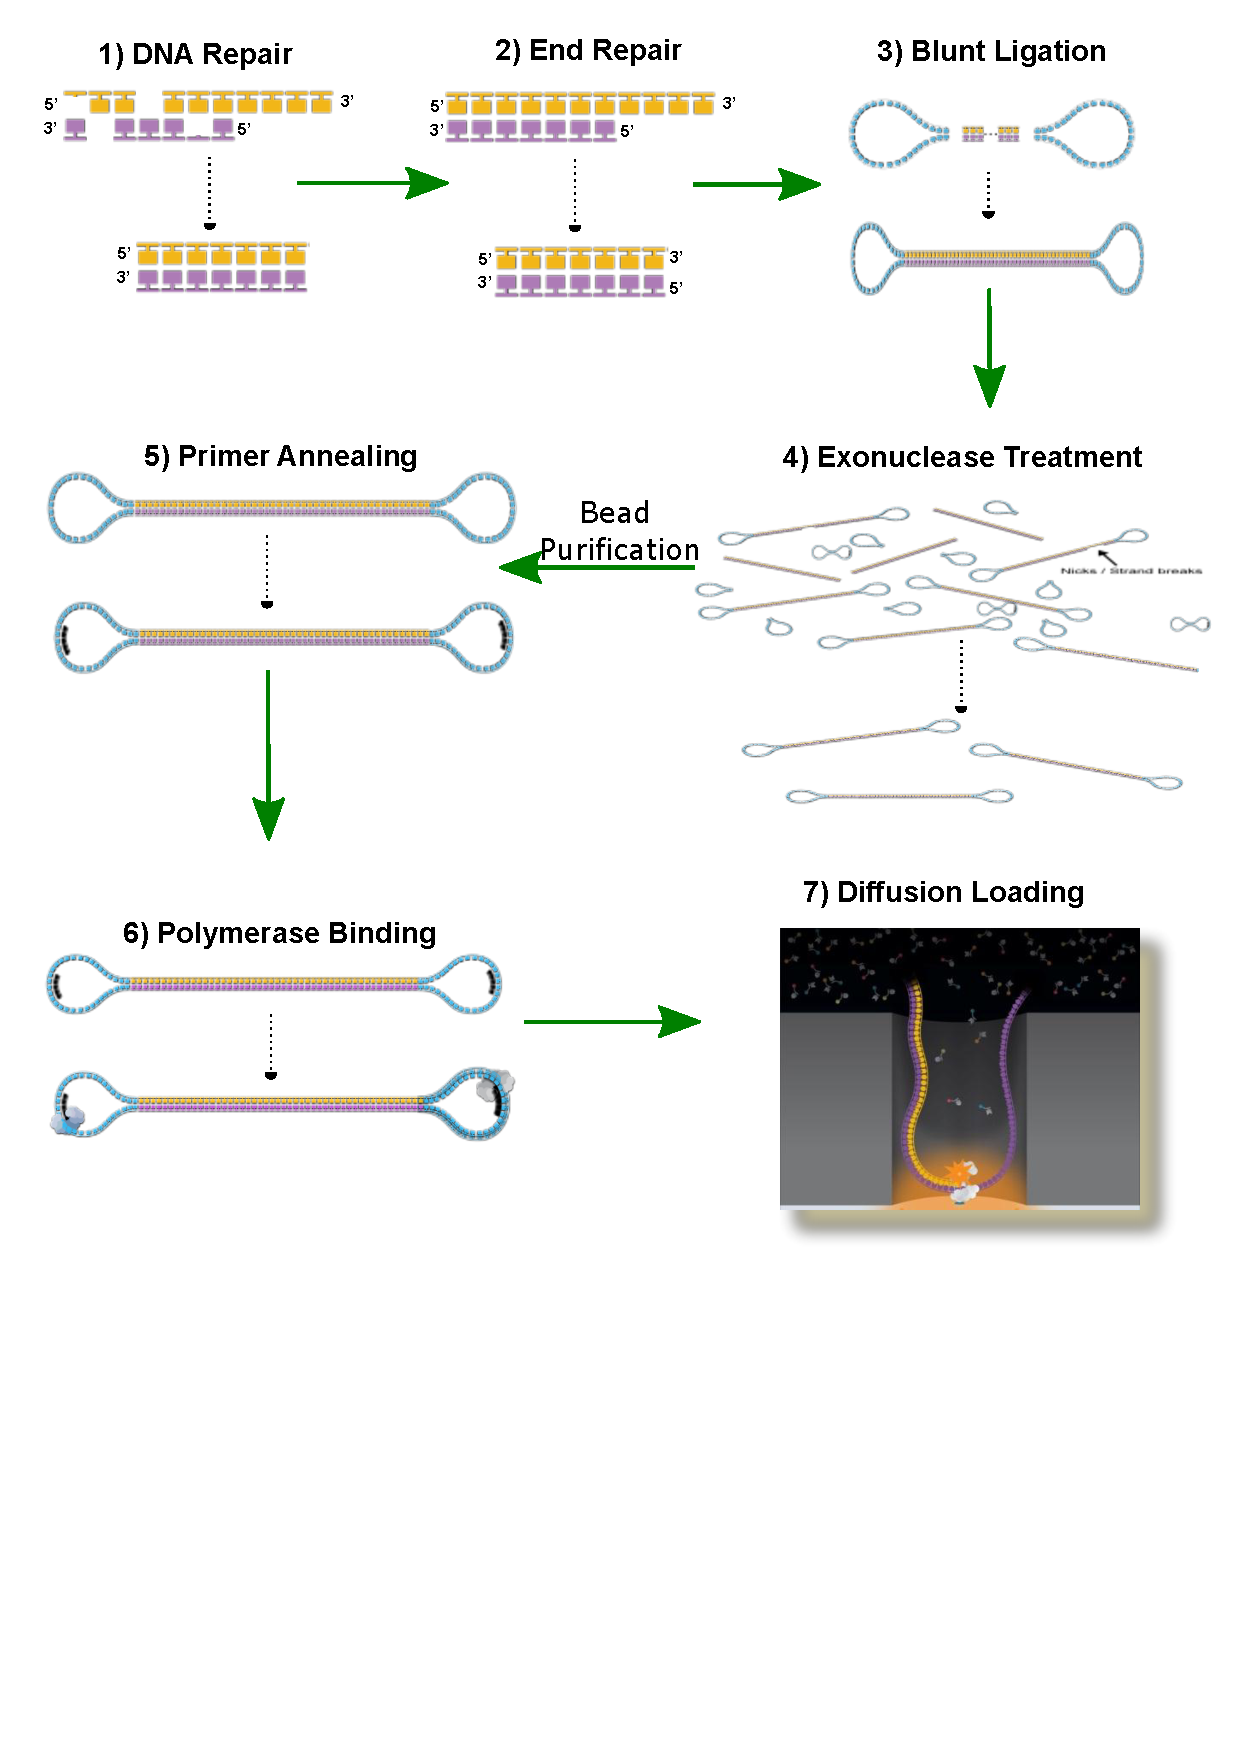
\includegraphics[page=1,trim={0cm 8cm 0cm 0cm},clip,scale = 0.70]{Figures/labwork_isoseq.pdf}
	\end{center}
	\captionsetup{width=0.95\textwidth,singlelinecheck=off}
	\caption[Lab workflow of Iso-Seq SMRT Bell Template Preparation, Primer Annealing \& Polymerase Binding]%
	{\textbf{Lab workflow of Iso-Seq SMRT Bell Template Preparation, Primer Annealing \& Polymerase Binding.} Shown is a flow diagram of the lab workflow of Iso-Seq library preparation for long-read sequencing on the Sequel:
		\begin{enumerate}
			\item Repair DNA Damages by repairing abasic sites and nicks, removing thymine dimers, oxidising guanines, deaminating cytosine; essential to ensure continuous sequence for uninterrupted polymerase processivity 
			\item Repair ends for blunt ligation with removal of 3' hangs and addition of 5' hangs by T4 DNA polymerase; essential for blunt ligation of SMRT bell adapters 
			\item Blunt Ligation by adding hairpin SMRT bell adapters to repaired ends
			\item Exonuclease treatment to remove incomplete SMRTbells with Exonuclease III and IV; essential to ensure sequencing of good library 
			\item Annealing of primer to both ends of the SMRT bell templates to initiate sequencing 
			\item Binding of polymerase to both ends of SMRT bell templates for efficient loading into ZMWs
			\item Immobilisation of polymerase-bound SMRTbells to ZMW by diffusion
			\\
		\end{enumerate} 
		Individual figures and legend are taken and adapted from "PacBio Sequel Library and Sequencing Preparation" presentation
	}
	\label{fig:isoseq_labworkflow}
\end{figure}

\subsection{Bioinformatics Pipeline} 
\label{section:isoseq_bioinformatics}

\begingroup
\parindent=0em
\etocsettocstyle{\rule{\linewidth}{\tocrulewidth}\vskip0.5\baselineskip}{\rule{\linewidth}{\tocrulewidth}}
\etocsetnexttocdepth{5}
\localtableofcontents 
\endgroup

\subsubsection{Introduction}
While the official PacBio bioinformatics tool for processing long Iso-Seq reads has been revised multiple times over the course of this research, the changes have been centred around three main sequential objectives to generate high-quality (HQ) isoforms \textit{de novo}, namely: 
\begin{enumerate}
	\item CCS: generate CCS from each sequencing ZMW
	\item Classify: identify full-length reads with primer removal
	\item Cluster: group reads derived from the same isoform to generate consensus sequence (high-quality full-length non-concatemer reads)	
\end{enumerate}
Bioinformatic analysis of Iso-Seq raw data can be performed using PacBio SMRT Link Suite (ref), a web-based end-to-end user interface. However, for optimisation of parameters and parallelisation of samples, an end-to-end command line was developed and used.  

\begin{figure}[h!]
	\centering
	\vspace{20pt}
	\includegraphics[page=17,trim={2cm 28cm 2cm 5cm},clip,scale = 0.8]{Figures/ProjectDevelopment_Figures.pdf}
	\captionsetup{width=0.95\textwidth}
	\caption[PacBio Iso-Seq Bioinformatics Pipeline]%
	{\textbf{PacBio Iso-Seq Bioinformatics Pipeline}: Pipeline is adapted from ToFU \nomenclature{ToFU}{Transcript isOforms: Full-length and Unassembled} \cite{Gordon2015}}
	\label{fig:isoseq_bioinformatics_Pipeline}
\end{figure}


Analysing long-read sequencing data requires a different approach to short-read, as the initial processing focuses on reducing the high error rate (due to low read coverage relative to short reads). Currently there were three methods of correcting long reads \cite{Zhao2019}: 
\begin{itemize}
	\item Hybrid error correction strategy using short-reads: LSC \cite{Au2012} which maps short reads, and LoRDEC which build De Brujin graph of short reads \cite{Salmela2014}
	\item Self-correction using long reads only: Long-read multiple aligner (LoRMA) \cite{Salmela2017}
	\item Reference-based correction by alignment of reads to reference genome by spliced-aware aligners: Minimap2. GMAP and STAR can also be used for alignment, however, they do not perform error correction during alignment and further capture non-canonical splice sites.  
\end{itemize}

Although the raw error rate of PacBio sequencing is 10-14\%, this is greatly reduced by the use of circular template and subsequent generation of circular consensus sequence. 

\subsubsection{Classify}
\label{section:classify}

\uline{\textbf{CCS Generation}}: In the first stage, the raw subreads (stored as a BAM file, unaligned.bam) from each “productive” ZMW were processed individually and collapsed to generate a CCS (Figure \cref{fig:Mechanism}\textbf{a}), according to: 
\begin{itemize}
	\item The number of full "passes" from the polymerase, and subsequently number of subreads generated; a full pass is defined by the presence of both SMRT adapters at both ends (Default: 3 passes)
	\item The minimum base accuracy across all subreads (Default: 99\%)
	\item Length of the subreads (Default: minimum 10 bases, maximum 21000 bases)
	\item Quality of subreads predicted by the CCS model (Default: Z-score of -3.5), and proportion of total subreads meeting the quality score (Default: \textgreater 30\%)
\end{itemize}

Across literature and PacBio scientific community, different parameter settings were recommended, particularly with \textit{number of full passes} and \textit{minimum base accuracy}, which had the greatest effect on the number of CCS reads generated for downstream analyses. Taking a subset of raw data from 10 randomised samples, a range of values across these two parameters were tested. CCS were then classified to full-length (FL, determined by the presence of 3'/5' primers and poly-A tail) and non-full-length (NFL) reads. 

\uline{\textbf{Lima}}: With successfully-generated CCS, cDNA primers and PacBio barcodes were identified and then removed using \textit{Lima}. CCS with unwanted orientations were removed and were oriented 5’ to 3’. A barcode score is calculated for each barcode pair (leading and trailing barcode), and is based on accuracy alignment to input cDNA primer sequences. The proportion of FL reads (number of FL reads over the number of CCS reads) varies on the insert transcript size; for Iso-Seq, a non-size selected library with a library distribution of 1-3kB typically has a 60-70\% FL. 

\uline{\textbf{Refine}}: Finally, full-length reads were refined by trimming of polyA tails, of a least a length of 20 bases, and removal of artificial concatemers to generate full-length non-chimeric (FLNC) reads. Artificial concatemers were defined as cDNA sequences with internal runs of polyA and polyT sequences, due to insufficient amount of blunt adapters during library preparation - this is typically low (<0.5\%). Conversely, it is challenging to differentiate and remove PCR-induced artificial chimera from true biological chimera. PCR-induced artefacts were defined as cDNA sequences that appear to be fusion transcripts, but were actually a result of non-optimal PCR reaction conditions. The number of FLNC reads should be very close to the number of FL reads, and any significant loss implicates issues at the SMRT bell library preparation.
Note Tama works on FLNC reads from Classify 

\subsubsection{Cluster}
In the second stage, Iso-Seq uses an iterative isoform-clustering algorithm (ICE – iterative clustering for error, called Quiver for PacBio RSII data and Arrow for Sequel data) to group all FLNC reads that were thought to be derived from the same isoform if: 
\begin{itemize}
	\item They differ less than 100bp on the 5’ end 
	\item Differ less 30bp on the 3’end 
	\item Do not contain internal gaps that exceed 10bp
\end{itemize}
By collapsing transcripts with differing 5' start [due to cDNA synthesis not preserving 5' end], some transcripts with alternative transcription start sites were lost while preserving those with alternative splicing and alternative polyadenylation. The representative transcript from those clustered is the longest one. 

A minimum of two FLNC reads were further required for a cluster. Consequently each FLNC read is classified to only one cluster, which is comprised of two or more FLNC reads. Two possible issues: reads belong to incorrect clusters, and reads that belong together were in separate clusters. [Briefly it first does clique-finding based on a similarity graph, then calls consensus using the Directed Acyclic Graph Consensus method and finally reassign sequences to different clusters based on their likelihood (Gordon et al. 2015)]. In previous Iso-Seq bioinformatic versions, FLNC reads were used to increase the coverage of each consensus isoform. However, with increasing throughput from Sequel I and II, this has been foregone. Cluster outputs the high-quality isoforms (HQ-isoforms), which have a consensus accuracy >=99\%. 

So in summary, each productive ZMW generates one polymerase read, which is collapsed to give a circular consensus sequence (CCS) assuming the requirements were met. CCS were then trimmed and processed for primer and poly-A sequence removal to generate full-length non-chimeric (FLNC) reads, which were clustered if they were thought to be derived from the same isoform. The number of associated full-length (FL) reads of each isoform therefore represents the number of ZMWs that sequenced the isoform of interest, and can infer abundance of mRNA isoform. However, Iso-Seq is only semi-quantitative due to preferential loading and sequencing bias of shorter fragments. It is worthy to note that all the steps up to now have been processed without a reference genome or transcriptome. 


Iso-Seq Versions 
In response to a much higher experimental throughput of Sequel compared to RSII, each subsequent   version of the official PacBio Iso-Seq tool saw a reduction in runtime, but an improvement of sensitivity to recover transcripts and specificity to reduce artefacts.

Iso-Seq 1 	
Iso-Seq 2	


In previous versions of official PacBio Iso-Seq tool, non-FLNC reads were re-incorporated at this stage to polish the consensus isoforms. Short reads from RNA-Seq can also be incorporated for error correction using various tools such as LoRDEC, LSC and Proovread. 

Since the introduction of Iso-Seq protocol, 3 versions of the informatics pipeline has been developed. Iso-Seq2 has an extra pre-clustering step to bin full length non-chimeric reads based on gene families. The latest version Iso-Seq3 is used in response to the much higher throughput of Sequel compared to RSII by using faster clustering algorithms. Using a more conservative primer removal and barcode demultiplexing step (with tool named LIMA), the Iso-Seq3 pipeline generates fewer but higher quality polished transcripts. 

High confidence transcripts can be determined by 1) presence of open reading frame (ORF), CDS length, interpro domain coverage, annotation edit distance 

\subsubsection{Genome/Transcriptome Alignment} 
High quality isoforms were then aligned to the reference genome (as opposed to transcriptome as otherwise miss novel isoforms using BLASR) using splice-awwere aligner Minimap2. Various long-read studies have used Minimap2 and GMAP (Križanovic et al. 2018 demonstrated marked success of GMAP vs other RNA-Seq Aligners). Tang et al. 2020, using subset of Oxford Nanopore reads evaluated number of splice sites mapped relative to known junctions, found Minimap2 to be more precise than GMAP. 

Using the –secondary=no parameter restricts the output to the best alignment, -x splice assumes read orientation relative to transcript strand unknown, and thus tries two rounds of alignment to infer orientation. As a splice-aware alignment, -x splice prefers GT[A/G]…[C/T]AG over GT[C/T]…[A/G]AG over other splicing signals (main donor/acceptor motifs). –u f forces Minimap2 to consider forward transcript strand only for alignment, slightly improving accuracy. –c 5 to accept non-canonical GT/AG splice junctions. 

--splice-flank=yes for human/mouse data in reads with relatively high sequencing error rate (necessary for ONT), but not for high quality IsoSeq reads (99\% - 100\%). 

\subsubsection{Genome Mapping}
HQ-isoforms from the pooled dataset were aligned to mouse genome using Minimap2, and a total of XXX reads (XX\%) were mapped. Errors for substitution, insertion and deletion were X\%, X\% and X\% respectively. XX\% of transcripts (polished) could not be mapped to reference genome, thus representing genes that fall into gaps in the assembly (mouse genome should be quite updated though)


\subsubsection{ERCC}
One source of error from long-read sequencing can occur at reverse transcription (RT)\nomenclature{RT}{Reverse Transcription}, whereby a premature termination in reverse transcription enzyme can result in a full-length cDNA, that is mistaken for a true isoform. To measure the degree of this technical error, ERCC, with known start and end positions can be used as benchmark. As detailed in \cite{Karlsson2017}, most ERCC reads fell within +/- 5bp at both 5' and 3' ends, with 3' end slightly more accurate than 5' end. From \cite{Sharon2013}, drop in read length was observed for ERCC for molecules longer than 1.5kb (PacBio RSII). Interestingly, non-coding exon junctions were more variable than coding-exon junctions, suggesting that codon exon splicing has a stricter control with refined splice donor/acceptor sites (\cite{Karlsson2017}) 
Of note, however, that while ERCC has been used as a standard for RNA-Seq method validation, the longest molecule is only ~2kB, thus limiting is usage to validate longer molecules. Given that XX of RNA transcripts in human and mouse transcriptome were >2kB, there is a need for longer control sequences. 

To assess the sensitivity across Iso-Seq runs to detect ERCC, a merged analysis of whole transcriptome samples (n = 10, WT = 5, TG = 5) was performed with ERCC alignment and further collapse using Cupcake. The counts of full-length transcripts pertaining to each sample were then obtained using a custom demultiplexed script, which classifies and counts the merged data based on the unique sequencing run id. Post SQANTI annotation and filtering, only a third of ERCC (unique number of ERCC = 37, 40.22\%) were identified from both WT (mean number of ERCC: 32.4 (35\%)) and TG (mean number of ERCC: 32.2 (35.22\%)), with no difference in number of ERCC detected between WT and TG, although there were some ERCC that were detected in WT but not in TG, and vice versa. A minority of ERCC (n = 8, 8.7\%) at higher concentration were further annotated with more than one "isoform", indicating the presence of technical artefacts and more stringent filtering or clustering required, with ERCC at a higher concentration more likely to be sequenced and annotated with multiple redundant "isoforms". Exploration of these "isoforms" revealed them to be shorter transcripts likely to be generated as a result of fragmentation of the original molecule, incomplete PCR synthesis and template-switching. Application of TAMA-GO's script, Tama-remove-fragment-models.py, successfully removed these partial, redundant isoforms, while retaining the intact isoforms. 

Deeper investigation into the low coverage of ERCC further identified an additional 20 lowly-expressed ERCC that were discarded from cupcake's collapse scripts under the default coverage (alignment identity) parameters at 99\%. Exploration of these imperfect-aligned sequences revealed 5'prime degradation of XX-XX nucleotides - one of the limitations of not using a 5'cap protocol. Inclusion of these ERCC using a lower minimum coverage threshold at 95\% increased the number of ERCC detected by 20\% (unique number of ERCC = 57, 61.96\%), and strengthening the relationship between full-length read count and known amount of ERCC (95\% coverage: corr = 0.98, p = 1.41 x 10\textsuperscript{-41}; 99\% coverage: corr = 0.82, p = 4.89 x 10\textsuperscript{-10}).   


\subsubsection{Cupcake}
To avoid redundancy of transcripts, aligned and filtered HQ transcripts were further collapsed to obtain a final set of unique, full-length, high-quality isoforms using Cupcake (a set of publicly-available, supporting scripts). HQ transcripts were filtered out for lack of mapping and low coverage/identity before collapsing into unique isoforms.  

The abundance of each unique isoform can be estimated from the number of associated FL and NFL reads during Iso-Seq cluster (not accounting for HQ transcripts that have been filtered out).  Finally, isoforms were filtered by 5’degradation due to the lack of a cap protection employed in the cDNA synthesis step (Clontech SMARTer cDNA kit). 

\subsubsection{Validation of isoforms with RNA-Seq} 
\label{section:ch2_rnaseq_support_bioinformatics}
Samples sequenced with paired-end reads, Illumina Hi-Seq, 125bases. Paired end reads as more accurate for identifying and sequencing junctions. RNA-Seq data through stringent filtering (plot of fastqc) and aligned to mouse genome (Gencode, version X) using STAR (see section X for parameters). Abundance in TPM was then calculated with Kallisto (v0.46.0) \cite{Bray2016} as an input into SQANTI to identify coverage of splicing junctions with RNA-Seq.  

Provides support of transcripts from RNA-Seq data, highest expression of RNA-Seq reads of the splice junctions 
The junction with lowest coverage from RNA-Seq, and its associated read count 	
Standard deviation of read counts across all the junctions for each transcript 


\subsubsection{SQANTI2 classification and filtering of isoforms} 
\label{sec:sq_exp}
High-quality, clustered, filtered isoforms from Cupcake were characterised using SQANTI2 (v7.4), a pipeline initially developed by Conesa et al. [ref] and refined by Elizabeth Tseng (Pacific Bioscience’s specialist) [ref].
In combination with genome annotation, SQANTI2 performs a reference-based correction of sequences and classifies isoforms based on splice junctions. The curated transcriptome can be further filtered and annotated with public datasets and RNA-Seq data (Section \ref{section:ch2_rnaseq_support_bioinformatics}). Public datasets include 
\begin{itemize}
	\item FANTOM5 Cap Analysis of Gene Expression (CAGE) peaks: map transcripts, transcription factors, transcriptional promoters and enhancers
	\item Intropolis\cite{Nellore2016} : a comprehensive human RNA-Seq dataset
	\item PolyA motifs 
\end{itemize}


\boldheader{Transcriptome Annotation and Isoform Classification}
\label{section: sqanti_annotations}
Using SQANTI classifications based on splice junctions, the transcriptome was segregated into the following categories (Figure \ref{fig:sqanti_cate}): 
\begin{itemize}
	\item Well-known annotated genes with known isoforms, further isoforms classified as
	\begin{itemize}
		\item Full Splice Match (FSM) if reference and query isoform have the same number of exons with matching internal junction. The 5’ and 3’ end, however, can differ 
		\item Incomplete Splice Match (ISM) if query isoform has fewer 5’ exons than the reference, but the 3’ exons and internal junctions match. The 5’ and 3’ ends can also differ 
	\end{itemize}
	\item Well-known annotated genes with novel isoforms, with isoforms classified as
	\begin{itemize}
		\item Novel in Catalogue (NIC) if query isoform has different number and combination of exons to reference isoform, but is using a combination of known donor/acceptor splice sites 
		\item Novel Not In Catalogue (NNC) if query isoform has different number and combination of exons to reference isoform like NNC, but also has at least one unannotated/novel donor or acceptor site
		\item Genic Intron: the query isoform is completely contained within an annotated intron.
		\item Genic Genomic: the query isoform overlaps with introns and exons.
	\end{itemize}
	\item Unannotated, novel genes with novel isoforms with isoforms classified as
	\begin{itemize}
		\item Antisense: the query isoform does not have overlap a same-strand reference gene but is anti-sense to an annotated gene.
		\item Intergenic: the query isoform is in the intergenic region
	\end{itemize}
\end{itemize}

Based on the pair of dinucleotides framing the intron boundary, splice junctions were either categorised as canonical for GT-AG, GC-AG and AT-AC and all the other possible combinations as non-canonical.  

Lastly it can provide further classification of transcripts:  
As protein-coding or non-protein-coding by the presence of coding sequence
that may potentially undergo non-sense medicated decay by the presence of ORF but CDS ends before the last junction
that contain one or multiple exons (mono-exonic or multi-exonic respectively)
that contain intronic sequences (intron retention) 
as fusions. The criteria XXXX

\begin{figure}[htp]
	\begin{center}
		\includegraphics[page=3,trim={2cm 28cm 2cm 5cm},clip,scale = 0.8]{Figures/ProjectDevelopment_Figures}
	\end{center}
	\captionsetup{width=0.95\textwidth}
	\caption[Isoform Classifications by SQANTI]%
	{\textbf{Isoforms were classified by SQANTI as novel or known, and annotated to novel or known genes based on splice junctions}. An isoform was classified as ‘FSM’ if it aligned with reference genome with the same splice junctions and contained the same number of exons, ‘ISM’ if it contained fewer 5’ exons than the reference genome, ‘NIC’ if it represented a novel isoform containing a combination of known donor or acceptor sites, or ‘NNC’ if it represented a novel isoform with at least one novel donor or acceptor site. FSM – Full splice match, ISM – Incomplete splice match, NIC – Novel in catalogue, NNC – novel not in catalogue}
	\label{fig:sqanti_cate}
\end{figure}


\boldheader{Further filtering of isoforms from technical artefacts}
SQANTI was further used to filter the curated transcriptome from any technical artefacts that were generated during library preparation, including artefacts from RT template switching (TS \nomenclature{TS}{Template Switching}) and off-priming \cite{Conesa2016} (Figure \ref{fig:lib_prep_artifacts}. RT template switching is an intrinsic feature of RT whereby the enzyme can transit within (intramolecular TS) or across (intermolecular TS) DNA templates without terminating cDNA synthesis, if the original DNA template harbours two or more direct repeats \cite{Cocquet2006}. This can result in either chimeric cDNAs or short, incomplete cDNAs that can be misinterpreted as isoforms generated from non-canonical splicing \cite{Houseley2010} (Figure \ref{fig:lib_prep_artifacts}a). Capitalising on the fact that RT switching is homology-dependent, SQANTI can identify these RT-switching artefacts by finding these direct repeats \cite{Conesa2016}. 

Finally, off-priming artefacts can be generated from the binding of oligo(dT) primer to other internal homo-polymeric adenines (A) regions that can be located within cDNA template, and thereby generate truncated cDNAs \cite{Nam2002} (Figure \ref{fig:lib_prep_artifacts}b). SQANTI can explore the likelihood of thee events by determining the percentage of adenines (A) within the 20 nucleotide window downstream from the genomic coordinates of the isoform 3'ends and remove any that have a percentage lower than the user-defined threshold \cite{Conesa2016} - the lower the percentage of As, the higher the likelihood of the presence of internal polyA and off-priming. 

\begin{figure}[h]
	\begin{center}
		\includegraphics[page=4,trim={2cm 21cm 0 1cm},clip, scale = 1]{Figures/ProjectDevelopment_Figures.pdf}
	\end{center}
	\captionsetup{width=0.95\textwidth}
	\caption[Technical artefacts generated during library preparation and identified in SQANTI]%
	{\textbf{SQANTI identifies technical artefacts that were generated during first-strand cDNA synthesis a)}: Schematic diagram of reverse transcription template switching, taken from Cocquet et al.(2006) \cite{Cocquet2006}. The black and blue line represent the original cDNA and synthesising cDNA from RT respectively, the black box represent the direct repeats and the light grey sphere represent the RT enzyme. As exemplified, RT template switching is further facilitated by RNA secondary structures that could bring the repeats into proximity \cite{Cocquet2006}. \textbf{b)} Schematic diagram of off-priming of oligo(dT) primer to internal A repeats, taken from Nam et al. (2002) \cite{Nam2002}. Oligo(dT) primer from first-strand cDNA synthesis can anneal to internal poly(A) sequence rather than the 3'end polyA, resulting in two truncated cDNAs.}
	\label{fig:lib_prep_artifacts}
\end{figure}

%This was developed to remove artifacts from library preparation: i.e. intrapriming of polyA that usually happens in antisense strands and also lack of junction support in NNC; increase \% of FSM transcripts, and removes NIC. 

In summary, the isoforms were filtered by the following criteria: 
\begin{enumerate}
	\item FSM with a reliable 3’ end by:
	\begin{itemize}
		\item >60\% of As in transcription termination site and no detected polyA motif, indicative of genomic contamination
		\item <Xbp 5' start and 3’ end to reference transcript start end
	\end{itemize}
	\item Any other transcripts that have a reliable 3' end do not have any splice junctions were annotated as Reverse Transcription Switching. 
\end{enumerate}

\subsubsection{Isoform Quantification}
Isoform abundance was determined in two ways, using either a hybrid approach of long and short reads or the normalised full-length long read count as proxy (\cref{fig:isoform_quant_strategy}). The hybrid approach was a modified strategy of typical RNA-Seq quantitive analyses, whereby short reads were aligned to the Iso-Seq defined transcriptome (a merged, comprehensive annotation) rather than the reference genome, thereby improving read alignment to condition-specific transcripts and enabling the detection of novel transcripts. 


\begin{figure}[htp]
	\begin{center}
		\includegraphics[page=8,trim={2cm 19cm 0 1cm},clip, scale = 0.8]{Figures/ProjectDevelopment_Figures.pdf}
	\end{center}
	\captionsetup{width=0.95\textwidth}
	\caption[Strategies for isoform quantification]%
	{\textbf{Strategies for isoform quantification using long and short reads}: A schematic diagram of three strategies adopted for determining isoform abundance, using either short RNA-Seq reads aligned to the reference genome or the Iso-Seq defined transcriptome (hybrid approach), or the normalised full-length read count directly from long reads}
	\label{fig:isoform_quant_strategy}
\end{figure}


\boldheader{Removal of ISM and merging of FSM}
Following \textit{SQANTI} annotations, there were many examples where multiple ISM and several FSM transcripts were annotated to the same known isoform (exemplified in \cref{fig:redudant_sncatranscripts}). This is likely due to varying extent of 5'degradation and truncation - small degree of degradation or truncation would result in differing 5' and 3' ends respectively while preserving the internal exonic structure and thereby generating several FSM; conversely, a large degree of degradation or truncation would generate smaller partial isoforms that also have matching, albeit smaller overlap, exonic structure. To ease downstream quantitative analyses, ISM and shorter FSM were assumed as partial products of the longest detected FSM transcript, and the associated counts were aggregated (as shown in \cref{fig:ism_collapse}). However, there is a caveat that significantly shorter ISM transcripts could in theory be mapped to multiple isoforms.  

\begin{figure}[htp]
	\begin{center}
		\includegraphics[page=10,trim={0cm 0cm 0 0cm},clip, scale = 0.7]{Figures/ProjectDevelopment_Figures.pdf}
	\end{center}
	\captionsetup{width=0.95\textwidth}
	\caption[Redundant ISM and FSM associated with same known isoform]%
	{\textbf{Redundant ISM and FSM associated with known transcript of \textit{Snca}}: \textbf{a)} Visualising transcripts using \textit{Swan}, shown are \textbf{b)} transcripts detected after \textit{SQANTI} annotation of the mouse transcriptome using the targeted approach. An example of detecting multiple redundant transcripts annotated to the same isoform, all the transcripts depicted were annotated to ENMUST0000014268.4 which typically differed at the 5' and 3' end.}
	\label{fig:redudant_sncatranscripts}
\end{figure}

\begin{figure}[htp]
	\centering
	\includegraphics[page=9,trim={0cm 12cm 0cm 0cm},clip,scale = 0.8]{Figures/ProjectDevelopment_Figures.pdf}
	\captionsetup{width=0.95\textwidth,singlelinecheck=off}
	\caption[Merging of ISM and FSM]%
	{\textbf{Merging of ISM and FSM associated with the same known isoform}. All illustration of handling with multiple ISM and FSM associated with the same known transcript. In this example, 6 isoforms were detected for "Gene 1", however, only 4 known isoforms were identified (denoted as ENMUST1-4). For ease of annotation and quantification, ISM and shorter FSM were assumed partial products of the longer FSM. Consequently, in the case where: 
		\begin{itemize}
			\item both ISM (PB.1.2) and FSM (PB.1.1) are annotated to the same transcript (shaded green), the FSM takes precedence as the associated transcript and counts from respective ISM are aggregated 
			\item there is one ISM (PB.1.3) but no corresponding FSM for the associated transcript (shaded blue), the ISM is retained
			\item there are multiple ISM (PB.1.4, PB.1.5) annotated to the same transcript (shaded orange), the longest ISMs (PB.1.5) takes precedence and counts from respective ISM are similarly aggregated 
			\item there are multiple FSM (PB.1.6, PB.1.7) annotated to the same transcript (shaded purple), the longest FSM (PB.1.7) takes precedence and counts are similarly aggregated
			\\
		\end{itemize} 
		PB - PacBio. FSM - Full Splice Match, ISM - Incomplete Splice Match, FL - Full-length read counts.  
	}
	\label{fig:ism_collapse}
\end{figure}

\clearpage
\boldheader{RNA-Seq Alignment to Iso-Seq defined transcriptome}
For the hybrid approach of aligning short reads to Iso-Seq defined transcriptome from the targeted approach, several factors were optimised including the library size and the Iso-Seq annotation (\cref{tab:rnaseq_alignment_targeted}) to align RNA-Seq reads to targeted transcriptome dataset using \textit{Kallisto}. 

\begin{table}[h]
	\centering
	\caption[RNA-Seq Alignment strategy to Iso-Seq defined targeted transcriptome]%
	{\textbf{RNA-Seq Alignment strategy to Iso-Seq defined targeted transcriptome}. Tabulated is trialled methods of aligning short reasd to Iso-Seq defined transcriptome, with alterations either of the sequencing library (such as the pool of the sequencing reads for alignment) and the choice of Iso-Seq isoform for alignment}
	\label{tab:rnaseq_alignment_targeted}
	\begin{threeparttable}
		\begin{tabular}{@{}cll@{}}
			\toprule
			Method & Sequencing Library                       & Annotation                            \\ \midrule
			1      & Targeted Transcriptome (All Reads)\tnote{a}       & No Isoform collapse\tnote{c}                   \\
			2      & Targeted Transcriptome (All Reads)\tnote{a}       & Isoform collapse to longest FSM\tnote{d}       \\
			3      & Targeted Transcriptome (All Reads)\tnote{a}       & Isoform collapse to most abundant FSM\tnote{e} \\
			4      & Targeted Transcriptome (On-Target Reads)\tnote{b} & Isoform collapse to longest FSM\tnote{d}       \\
			5      & Targeted Transcriptome (On-Target Reads)\tnote{b} & Isoform collapse to most abundant FSM\tnote{e} \\
			6 & \begin{tabular}[c]{@{}l@{}}Whole Transcriptome \& \\ Targeted Transcriptome (On Target Reads)\end{tabular} & Isoform collapse to longest FSM \\ \bottomrule
		\end{tabular}
		\begin{tablenotes}
			\footnotesize
			\item[a] Sequencing reads from on-target and off-target genes
			\item[b] Sequencing reads aligned only to on-target genes
			\item[c] Transcriptome annotation following \textit{SQANTI} with no removal of redundant ISM and FSM
			\item[d] Transcriptome annotation following \textit{SQANTI} with collapse of redundant ISM to respective longest FSM of same transcript and aggregated counts
			\item[e] Transcriptome annotation following \textit{SQANTI} with collapse of redundant ISM to respective most abundant FSM of same transcript and aggregated counts 
		\end{tablenotes}
	\end{threeparttable}
\end{table}

However, independent of the scaffold or library size, \textit{Kallisto} appeared to mis-assign short reads to novel isoforms. This is exemplified with \textit{Clu} (\cref{fig:Clu_TargetedRNAseqAlignment}) and \textit{Bin1} (\cref{fig:Bin1_TargetedRNAseqAlignment}).   Using total Iso-Seq FL reads from targeted transcriptome as proxy of transcript expression, the known and longer isoforms associated with both \textit{Clu} (\cref{fig:Clu_TargetedRNAseqAlignment}\textbf{a}) and \textit{Bin1}(\cref{fig:Bin1_TargetedRNAseqAlignment}\textbf{a}) were most abundant whereas the novel isoforms were only lowly detected. Conversely, alignment of RNA-Seq reads to targeted transcriptome often ascribed the novel isoforms as the dominant isoform(s), particularly when further collapsing targeted transcriptome to longest or most abundantly expressed isoforms or limiting the scaffold to only on-target reads (Methods 2 - 5 from \cref{tab:rnaseq_alignment_targeted}). Nonetheless, while using all the reads from the targeted transcriptome with redundant ISM and FSM is more likely to ascribe the known isoform as the dominant isoform, mis-asignment can still occur with the shorter, redundant ISM annotated as most abundantly expressed rather than the longer, complete FSM (\cref{fig:Clu_TargetedRNAseqAlignment}\textbf{a, b, d}).

Visualisations of the dominant known isoform ascribed by Iso-Seq FL read counts and the dominant novel isoform ascribed by RNA-Seq alignment from \textit{Clu} and \textit{Bin1} show that both isoforms are structurally very similar, with almost identical internal exonic structure bar one or two exons with differing splice junctions. There was no difference in RNA-Seq coverage from \textit{Kallisto} alignment to targeted transcriptome across all the methods \cref{tab:rnaseq_alignment_targeted}), suggesting that the issue is the probabilistic assignment of reads to isoforms (Expectation-Maximum algorithm) rather than the alignment. It appears that in cases where the known and novel isoforms are similar in transcript structure, and consequently there are only a few short reads that can be unambiguously assigned, \textit{Kallisto} fails to quantify at an isoform level. Given that significantly more novel isoforms are identified using the targeted approach than the whole transcriptome approach, this is more likely to be evident in the former.   


\newgeometry{left=0.5cm,top=1cm,right=0.5cm}
\begin{landscape}
	\begin{figure}[htp]
		\centering
		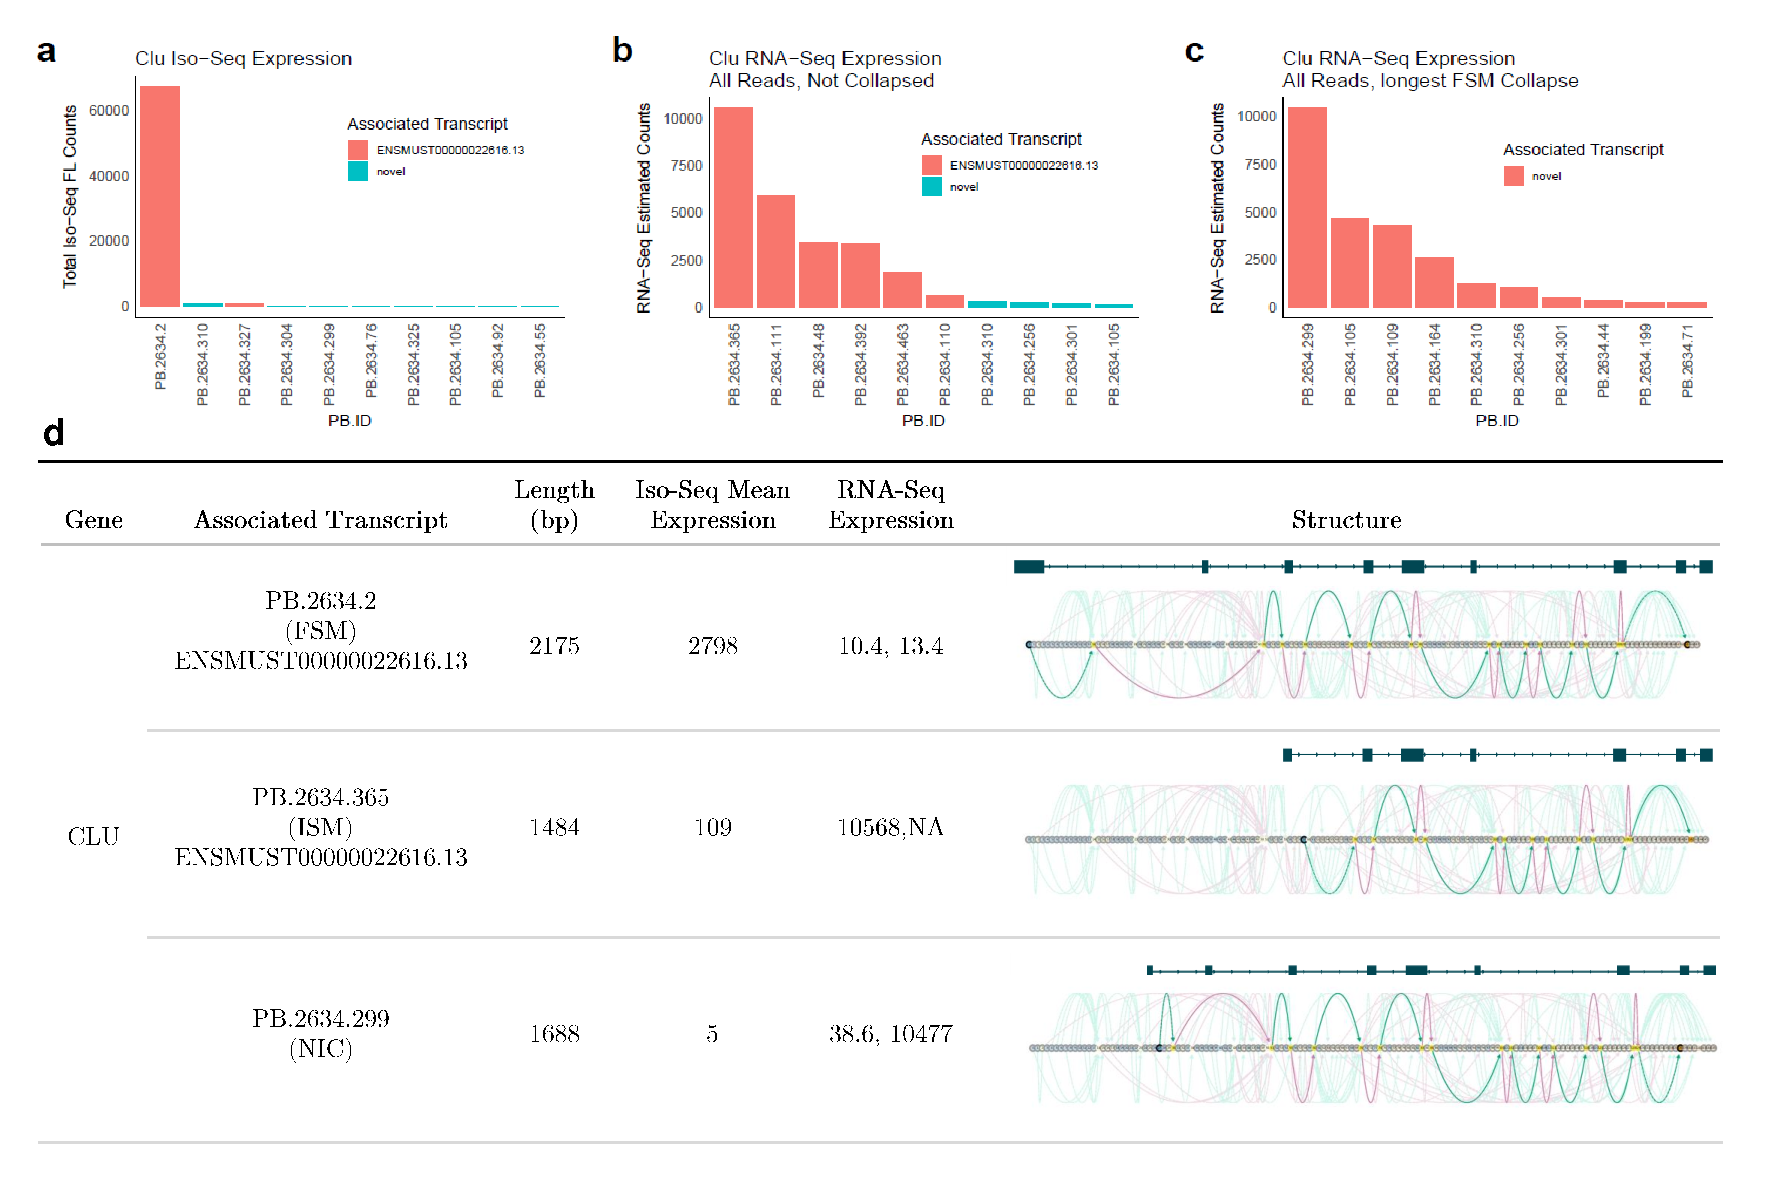
\includegraphics[page=1,trim={0cm 1cm 0cm 0cm},clip,scale = 0.8]{Figures/ProjectDevelopment_Figures_Landscape.pdf}
		\captionsetup{width=1.2\textwidth,singlelinecheck=off}
		\caption[RNA-Seq mis assignment of dominant isoform associated with \textit{Clu}]%
		{\textbf{RNA-Seq mis assigns \textit{Clu}'s novel isoform as most abundantly expressed}. Shown are the top 10 most abundantly expressed \textit{Clu} transcripts based on \textbf{a)} Iso-Seq full-length read counts from targeted transcriptome, \textbf{b)} RNA-Seq reads aligned to all reads in targeted transcriptome, with no further collapse of redundant FSM and ISM transcripts (Method 1 in \cref{tab:rnaseq_alignment_targeted}) and \textbf{c)} RNA-Seq reads aligned to all reads in targeted transcriptome with isoforms further collapsed to longest FSM (Method 2 in \cref{tab:rnaseq_alignment_targeted}). Of note, all other methods (3 - 6) generated a similar plot to figure c. \textbf{d)} Swan visualisations of most abundantly expressed isoforms according to respective methods. Iso-Seq mean expression refer to average full length read counts from targeted transcriptome. RNA-Seq mean expression refer to estimated counts from \textit{Kallisto} in Figures b and c. 
		}
		\label{fig:Clu_TargetedRNAseqAlignment}
	\end{figure}
	
	
	\begin{figure}[htp]
		\centering
		\includegraphics[page=2,trim={0cm 0cm 0cm 0cm},clip,scale = 0.8]{Figures/ProjectDevelopment_Figures_Landscape.pdf}
		\captionsetup{width=1.2\textwidth,singlelinecheck=off}
		\caption[RNA-Seq mis-assignment of dominant isoform associated with \textit{Bin1}]%
		{\textbf{RNA-Seq mis-assigns \textit{Bin1}'s novel isoform as most abundantly expressed}. Shown are the top 10 most abundantly expressed \textit{Bin1} transcripts based on \textbf{a)} Iso-Seq full-length read counts from targeted transcriptome, \textbf{b)} RNA-Seq reads aligned to all reads in targeted transcriptome, with no further collapse of redundant FSM and ISM transcripts (Method 1 in \cref{tab:rnaseq_alignment_targeted}) and \textbf{c)} RNA-Seq reads aligned to all reads in targeted transcriptome with isoforms further collapsed to longest FSM (Method 2 in \cref{tab:rnaseq_alignment_targeted}). Of note, all other methods (3 - 6) generated a similar plot to figure c. \textbf{d)} Swan visualisations of most abundantly expressed isoforms according to respective methods. Iso-Seq mean expression refer to average full length read counts from targeted transcriptome. RNA-Seq mean expression refer to estimated counts from \textit{Kallisto} in Figures b and c. 
		}
		\label{fig:Bin1_TargetedRNAseqAlignment}
	\end{figure}
\end{landscape}
\restoregeometry

\subsubsection{Iso-Seq isoform expression}
To control for sequencing bias in library depth, full-length (FL) read count for each isoform is normalized to transcripts per million (TPM \nomenclature{TPM}{Transcripts per Million})), which is calculated as: 

\begin{align*}
	FL\;\:TPM (x_{sample},y_{sample})=\frac{Raw\;\:FL\;\:count (x_{isoform},y_{sample})}{Total\;\:FL\;\:count (y_{sample})} *10^6
\end{align*}

With a cut-off lower than 0.5 TPM, a 0.5 - 10 TPM refers to low expression, a 11- 1000 refers to medium expression, and > 1000 TPM high expression [literature ref]. 

TPM is the most effective within-sample normalisation method to relatively quantify gene expression in a sample \cite{Abrams2019}. Other methods include RPKM (reads per kilobase of transcripts per million mapped reads), FPKM (fragments per kilobase of exon model per million mapped reads), which uses gene length to control for fragmentation in RNA-Seq protocol ("effective length normalisation") - however, this is not necessary in Iso-Seq.  

Between-sample normalisation methods to relatively quantify expression of the same gene in different samples, remove technical variations due to presence of few highly expressed genes that make up a significant proportion of total reads, and due to different number of reads in each sample. 

\subsubsection{Limitations}
While PacBio's Iso-Seq have major potential for transcriptome annotation, there were currently several major limitations that need to be addressed with further development of library preparation and bioinformatic data analyses \cite{Kuo2017}: 
\begin{enumerate}
	\item Lack of normalisation of RNA libraries, resulting in biased sequencing of high abundance transcripts and subsequent over-representation of such transcripts 
	\item Degradation of transcripts from 5' end, and thus lack of confidence in transcription start site and full-length structure 
\end{enumerate}

Despite the ability of long-read sequencing (particularly, Iso-Seq\nomenclature{Iso-Seq}{Isoform Sequencing}) to discover large number of novel and longer transcripts and identify complex splicing events such as alternative adenylation, there are inherent biases to sequencing the more highly-expressed and relatively shorter transcripts. Consequently, while the new chemistry has improved the error rate and increased throughput, the coverage is still insufficient for accurate transcript quantification and sensitive differential transcript analysis based on long reads alone (Koren et al., 2012). Furthermore, there is currently no consensus to validate or functionally characterise these transcripts (B. Wang, Kumar, Olson, \& Ware, 2019). The current standard for such application is thus a hybrid approach of aligning the short-reads to the long-reads to improve alignment and assemblage, and for downstream isoform quantification. 

Isoform-specific expression can be deduced from short-reads alone using statistical models if the gene is well annotated (i.e. all isoforms are known) based on i) reads aligning to contiguous genomic segment (exonic reads) and ii) reads aligning to two contiguous segments with a single gap of 60-400bp (junction reads)(Jiang and Wong, 2009)).

Various bioinformatic tools and computational models have been developed to quantify isoform quantification from RNA-Seq data. There are currently two main methods:
\begin{enumerate}
	\item Inclusion level, calculated for a regulated exon by aligning reads either to candidate alternative exons and its junctions (inclusion reads), or to flanking exons and subsequently skipping the candidate alternative exon (skipping/exclusion reads) (Chen et al. 2012)
	\item Percent-Spliced-In (PSI\nomenclature{PSI}{Percent-Spliced In}), calculated by proportion of isoforms that include the exon (Venables et al. 2008)(Katz et al. 2010). If the PSI value is calculated for a particular splicing event, it can be considered equivalent to the inclusion level. 
\end{enumerate}
Isoform quantification can either be expressed as a global measure of expression, which provides a global gene expression ranking in one sample (measured by RPKM: Reads of a transcript sequence per Millions mapped read\nomenclature{RPKM}{Reads of a transcript sequence per Millions}), or as a relative measure of expression, which is normalized per gene locus and comparable across conditions (measured by inclusion level or PSI value). 

Isoform abundance calculated by aligning short-reads to transcriptome is preferential to alignment with reference annotation library (RefSeq/GENCODE) in narrowing down the isoforms expressed and thus subsequently enabling more reliable abundance quantification. Reference annotation library is constructed on all data from the same species, and inclusion of annotated but not truly expressed isoforms can increase variability of abundance estimates. Finally, if the reference library is incomplete, then truly expressed isoforms would be completely missed and RNA-Seq reads would be incorrectly assigned to annotated isoform (\cite{Au2013})


\textbf{Differential Isoform Usage }\\
\label{intro:dtu}
When analyzing splicing patterns between multiple conditions, changes in isoform abundance can be defined in two ways: 
\begin{enumerate}
	\item Differential Isoform Expression (DIE\nomenclature{DIE}{Differential Isoform Expression}): changes in absolute expression of an isoform, evaluated using count matrices 
	\item Differential Isoform Usage (DIU\nomenclature{DIU}{Differential Isoform Usage}): changes in relative expression of an isoform from the same gene, resulting in a change in isoform proportion and is evaluated using changes in gene exon usage	
\end{enumerate}

Figure X shows an example of a change in DIE but no change in DS: A two-fold increase of both isoforms from the same gene results in a change in absolute but not relative expression to one another. A change in DIE but not in DS may indicate a transcription-related mechanism. If a change in DS is observed, a change in DIE of one of the isoforms would also be observed. A change in multiple isoforms would also be observed, as long as the change is not in the same direction (upregulated/downregulated) with the same magnitude. Any changes in DS/relative abundance of isoforms indicate a splicing-related mechanism. 

In addition to exploring differential splicing in terms of isoform abundance, which typically involves an exon-based approach that focuses on differential exon usage (i.e. DEXSeq), a splicing based approach can also be taken. This involves analysing individual splicing events (exon skipping, alternative donor and acceptor) for systematic changes between conditions. rMATS, SUPP2, LeafCutter and Majiq are such tools that identify and quantify splicing events using junction reads. 

